\documentclass[bibtotoc,liststotoc,BCOR=5mm,DIV=12]{scrbook}

% use this declaration to set specific page margins
%\usepackage[a4paper , lmargin = {2.7cm} , rmargin = {2.9cm} , tmargin = {2.7cm} , bmargin = {4.6cm} ]{geometry}
\usepackage[a4paper]{geometry}

\usepackage{graphicx}
\usepackage{amsmath}
\usepackage{appendix}
\usepackage{amsthm}
\usepackage{amssymb}
\usepackage{algorithm}
\usepackage{algorithmic}

\usepackage[ngerman, english]{babel}
\usepackage{bibgerm}       		% german references
\usepackage[T1]{fontenc} % german characters
\usepackage{graphicx} 				% it's recommended to use PDF images but you can use JPG or PNG as well
\usepackage{url}           		% format URLs
\usepackage{hyperref} 				% create hyperlinks
\usepackage{listings, color}	% for source code
\usepackage{subfig}						% two figures next to each other (example: figure 3a), figure 3b)
\usepackage{scrlayer-scrpage}					% header and footer line
\usepackage{todonotes}
% header and footer line - no header & footer line on pages where a new chapter starts
\pagestyle{scrheadings}
\ohead{Design and Implementation of X}
\ihead{Your Name}
\ofoot[]{\thepage}
\ifoot{Thesis, TU Berlin, Fachgebiet SC, 2024}

% Define the 'definition' environment
\newtheorem{definition}{Definition}

% set path where images are stored
\graphicspath{{./img/}}

%
% der Befehl \hypenation versteht keine Sonderzeichen, also weder ä
% noch "a noch \"a. Wörter die derartige Zeichen enthalten müssen
% direkt im Text getrennt werden, z.B. Wör\-ter
%
\hyphenation{te-le-com-muni-cation 
te-le-com-muni-cation-specific 
Te-le-kom-mu-ni-ka-tions-API} 					% use this file to set explicit hyphenations (doesn't seem to work correctly)

\begin{document}
% ---------------------------------------------------------------
\frontmatter
    \thispagestyle{empty}
\begin{center}

\vspace*{1.4cm}
{\LARGE \textbf{Technische Universität Berlin}}

\vspace{0.5cm}

{\large Scientific Computing\\[1mm]}

Fakultät II\\
Straße des 17. Juni 136\\
10623 Berlin\\
https://www.tu.berlin/math\\

\vspace*{1cm}


\includegraphics[width=4cm]{tu_logo}

\vspace*{1.0cm}

{\LARGE Master Thesis}\\

\vspace{1.0cm}
{\LARGE \textbf{Decomposition-Invariant Conditional Gradient}}\\
\vspace*{0.3cm}
{\LARGE \textbf{Method in Boscia Framework}}\\
\vspace*{1.0cm}
{\LARGE Wenjie Xiao}
\\
\vspace*{0.5cm}
Matriculation Number: 0461607\\
01.01.2020\\ % 	date of submission
\vspace*{1.0cm}

Supervised by\\
Prof. Dr. \\
Prof. Dr. \\

\vspace*{0.5cm}
Assistant Supervisor\\

\vspace{3cm}


\end{center}


    \thispagestyle{empty}
    \cleardoublepage
    
    
    \newpage

\thispagestyle{empty}

\begin{large}

\vspace*{6cm}

\noindent
Hereby I declare that I wrote this thesis myself with the help of no more than the mentioned literature and auxiliary means.
\vspace{2cm}

\noindent
Berlin, 01.01.2050

\vspace{3cm}

\hspace*{7cm}%
\dotfill\\
\hspace*{8.5cm}%
\textit{(Signature \todo{[your name]})}

\end{large}
 
    \thispagestyle{empty}
    \cleardoublepage
    
    
    \thispagestyle{empty}
\vspace*{1.0cm}

\begin{center}
    \textbf{Abstract}
\end{center}

\vspace*{0.5cm}

\noindent 
\\
\\
On the one hand this PDF should give a guidance to people who will soon start to write their thesis. The overall structure is explained by examples. On the other hand this text is provided as a collection of LaTeX files that can be used as a template for a new thesis. Feel free to edit the design.
\\
\\
It is highly recommended to write your thesis with LaTeX. I prefer to use Miktex in combination with TeXnicCenter (both freeware) but you can use any other LaTeX software as well. For managing the references I use the open-source tool jabref. For diagrams and graphs I tend to use MS Visio with PDF plugin. Images look much better when saved as vector images. For logos and 'external' images use JPG or PNG. In your thesis you should try to explain as much as possible with the help of images.
\\
\\
The abstract is the most important part of your thesis. Take your time to write it as good as possible. Abstract should have no more than one page. It is normal to rewrite the abstract again and again, so  probaly you won't write the final abstract before the last week of due-date. Before submitting your thesis you should give at least the abstract, the introduction and the conclusion to a native english speaker. It is likely that almost no one will read your thesis as a whole but most people will read the abstract, the introduction and the conclusion.
\\
\\
Start with some introductionary lines, followed by some words why your topic is relevant and why your solution is needed concluding with 'what I have done'. Don't use too many buzzwords. The abstract may also be read by people who are not familiar with your topic.
    \thispagestyle{empty}
    \cleardoublepage
    
    \thispagestyle{empty}
\vspace*{0.2cm}

\begin{center}
    \textbf{Zusammenfassung}
\end{center}

\vspace*{0.2cm}

\noindent 
Da die meisten Leuten an der TU deutsch als Muttersprache haben, empfiehlt es sich, das Abstract zusätzlich auch in deutsch zu schreiben. Man kann es auch nur auf deutsch schreiben und anschließend einem Englisch-Muttersprachler zur Übersetzung geben.
    \thispagestyle{empty}
    
    
    \tableofcontents
    \thispagestyle{empty}
    
    \todo[inline]{talk to your supervisor if this is needed}
    \listoffigures
    \thispagestyle{empty}
    
    \listoftables
    \thispagestyle{empty}
    
% --------------------------------------------------------------

\mainmatter % comment single chapters for faster compilation

    \chapter{Introduction\label{cha:chapter1}}

This chapter should have about 4-8 pages and at least one image, describing your topic and your concept. Usually the introduction chapter is separated into subsections like 'motivation', 'objective', 'scope' and 'outline'.

\section{Background\label{sec:background}}

Mixed-integer nonlinear optimization problems (MINLP) are optimization problems that include both integer and continuous variables and exhibit nonlinear relationships in the objective function or constraints. These types of problems frequently arise in applications such as supply chain optimization, portfolio optimization, network design, and energy systems. MINLP problems are known for their complexity due to the non-convex nature introduced by integer constraints and nonlinear functions.

Commonly used algorithms and methods for solving MINLP problems include branch-and-bound, branch-and-cut, and decomposition methods. Branch-and-bound and branch-and-cut methods systematically explore the solution space by dividing it into smaller subproblems, which are easier to solve. Decomposition methods, such as Benders decomposition and Dantzig-Wolfe decomposition, break the problem into more manageable subproblems that can be solved independently, improving computational efficiency. simpler components.

\section{Thesis Structure\label{sec:objective}}

What kind of problem do you adress? Which issues do you try to solve? What solution do you propose? What is your goal?
'This thesis describes an approach to combining X and Y... The aim of this work is to...'

\section{Scope\label{sec:scope}}

Here you should describe what you will do and also what you will not do. Explain a little more specific than in the objective section. 'I will implement X on the platforms Y and Z based on technology A and B.'

Conclude this subsection with an image describing 'the big picture'. How does your solution fit into a larger environment? You may also add another image with the overall structure of your component.

'Figure \ref{fig:intro} shows Component X as part of ...' 
\\
\begin{figure}[htb]
  \centering
  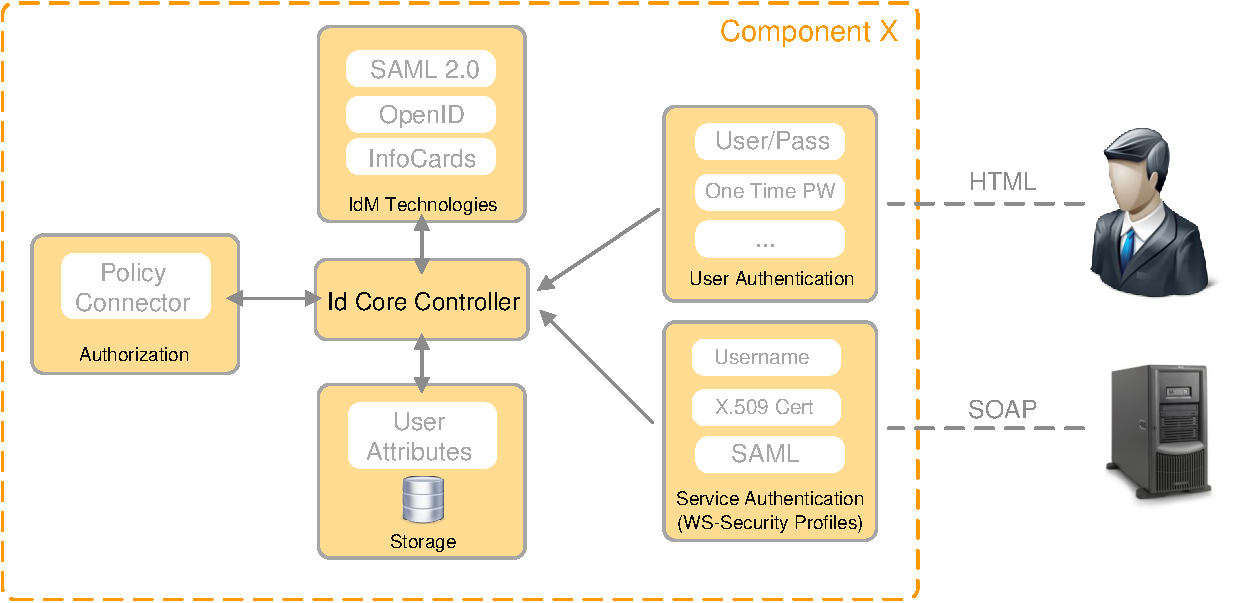
\includegraphics[width=9cm]{intro_example.pdf}\\
  \caption{Component X}\label{fig:intro}
\end{figure}

\section{Outline\label{sec:outline}}

The 'structure' or 'outline' section gives a brief introduction into the main chapters of your work. Write 2-5 lines about each chapter. Usually diploma thesis are separated into 6-8 main chapters. 
\\
\\
\noindent This example thesis is separated into 7 chapters.
\\
\\
\textbf{Chapter \ref{cha:chapter2}} is usually termed 'Related Work', 'State of the Art' or 'Fundamentals'. Here you will describe relevant technologies and standards related to your topic. What did other scientists propose regarding your topic? This chapter makes about 20-30 percent of the complete thesis.
\\
\\
\textbf{Chapter \ref{cha:chapter3}} analyzes the requirements for your component. This chapter will have 5-10 pages.
\\
\\
\textbf{Chapter \ref{cha:chapter4}} is usually termed 'Concept', 'Design' or 'Model'. Here you describe your approach, give a high-level description to the architectural structure and to the single components that your solution consists of. Use structured images and UML diagrams for explanation. This chapter will have a volume of 20-30 percent of your thesis.
\\
\\
\textbf{Chapter \ref{cha:chapter5}} describes the implementation part of your work. Don't explain every code detail but emphasize important aspects of your implementation. This chapter will have a volume of 15-20 percent of your thesis.
\\
\\
\textbf{Chapter \ref{cha:chapter6}} is usually termed 'Evaluation' or 'Validation'. How did you test it? In which environment? How does it scale? Measurements, tests, screenshots. This chapter will have a volume of 10-15 percent of your thesis.
\\
\\
\textbf{Chapter \ref{cha:chapter7}} summarizes the thesis, describes the problems that occurred and gives an outlook about future work. Should have about 4-6 pages.
    \chapter{Preliminaries\label{cha:chapter2}}
This section covers the preliminary concepts and assumptions used in this thesis, based on the DICG and Boscia papers.

\begin{definition}[Strongly convex function]
	A differentiable function \( f : \mathcal{X} \to \mathbb{R} \) is \( \mu\)-strongly convex if 
	\[
	f(y) - f(x) \geq \langle \nabla f(x), y - x \rangle + \frac{\mu}{2} \| y - x \|^2 \quad \text{for all } x, y \in \mathcal{X}.
	\]
\end{definition}

\begin{definition}[Smooth function]
	A differentiable function \( f : \mathcal{X} \to \mathbb{R} \) is  L-smooth convex if 
	\[
	f(y) - f(x) \geq \langle \nabla f(x), y - x \rangle + \frac{\L}{2} \| y - x \|^2 \quad \text{for all } x, y \in \mathcal{X}.
	\]
\end{definition}


\section{Assumptions from Boscia Paper \label{sec:assum}}
The Boscia framework makes the following assumptions:


\section{Problem Setting\label{sec:problem}}
Throughout this paper, we use \( \| \cdot \| \) to denote the Euclidean norm and we consider the optimization problem

\[
\min_{x \in \mathcal{P}} f(x),
\]

where we have following assumptions:\
\begin{enumerate}
	\item \(f(x)\) is \(\alpha\)-strong and \(\beta\)-smooth convex function with respect to the Euclidean norm.
	\item \(\mathcal{P}\) is a polytope with all vertices lying on the hypercube \( \{0, 1\}^n \).
	\item \(\mathcal{P}\) can be algebraically described as \(P = \{ x \in \mathbb{R}^n \mid x \geq 0, \, Ax = b \}. \)
\end{enumerate}

    \chapter{Framework\label{cha:chapter3}}
In this section, we outline the workflow for decomposition-invariant based mixed integer convex optimization over structured polytopes. We begin by introducing the Boscia Framework and the decomposition-invariant Frank-Wolfe algorithm, and then provide a detailed description of how these two methods are integrated.

\section{Boscia Framework\label{sec:boscia}}
The Boscia framework is designed to tackle large-scale mixed integer convex optimization problems by leveraging projection-free Frank Wolfe algorithm. It operates by breaking down a complex optimization problem into smaller, more manageable subproblems that can be solved independently and more efficiently. 

\subsubsection{Overview}
The Boscia framework provides a solution approach to MINLP, consisting of a branch-and-bound process over the convex hull of the feasible region with inexact node processing. This approach leverages the strengths of both the Frank-Wolfe (FW) algorithm and Mixed-Integer Programming (MIP) techniques to efficiently solve complex optimization problems.

At each node of the branch-and-bound tree, the FW algorithm solves the nonlinear subproblem over the convex hull of integer-feasible solutions, rather than over the continuous relaxation. This is achieved by solving a MIP as the Linear Minimization Oracle (LMO) within the FW process, which results in vertices of the integer hull. This innovative approach allows for stronger relaxations and a reduction in the size of the branch-and-bound tree.

Key features of this approach include:
\begin{enumerate}
	\item \textbf{Stronger Relaxations}: Optimizing over the convex hull of integer-feasible solutions instead of weaker continuous relaxations provides stronger relaxations, multiple feasible solutions at each node, and a reduced branch-and-bound tree size. This leads to more accurate and efficient solutions.
	
	\item \textbf{Error-Adaptive Solution Process}: The use of a FW-based error-adaptive solution process increases the amount of computation performed for higher accuracies, replacing exact convex solvers. This adaptive approach ensures that computational resources are allocated efficiently based on the required solution accuracy.
	
	\item \textbf{Warm-Starting}: Utilizing the active set representation of the solution at each node to warm-start the children iterates reduces the number of MIP solver calls. This technique significantly enhances computational efficiency by leveraging information from previously solved subproblems.
	
	\item \textbf{Lazification and Strong Branching}: The framework includes new lazification techniques and strong branching strategies that enhance the performance of the optimization process. Lazification techniques defer the solution of certain subproblems until necessary, while strong branching strategies improve the selection of branching variables.
	
	\item \textbf{Tightening Bounds}: Convexity and the FW gap are exploited to tighten bounds at each node, further reducing the search space. This bound tightening process improves the overall efficiency of the branch-and-bound method by reducing the number of nodes that need to be explored.
\end{enumerate}

This method avoids the issues associated with outer approximation approaches, such as reliance on near-feasible solutions and dense separation constraints, by using nonlinear relaxations and leveraging recent advances in FW and MIP methods to reduce the number of MIP subproblems. Unlike outer approximation methods, this approach maintains feasibility throughout the process and benefits from the flexibility of modern MIP solvers.

Extensive computational results demonstrate the effectiveness of this approach, showing significant improvements in solving large-scale MINLP problems. The Boscia framework is implemented as an open-source Julia package, Boscia.jl, which is available under the MIT license. This implementation allows researchers and practitioners to leverage the framework's capabilities in various applications, further validating its practicality and robustness.

\newpage

\begin{algorithm}[H]
	\caption{Boscia algorithm for Problem \eqref{1}}
	\label{alg:boscia}
	\begin{algorithmic}[1]
		\REQUIRE Primal-dual tolerance $\delta$, feasible set $\mathcal{X}$ as a boundable LMO, $\mathcal{J}$ the set of integer variables, objective $f$, initial point $v_0$, FW gap tolerance $\{\epsilon_t\}_{t \geq 0}$.
		\STATE $(l^0, u^0) \gets \text{global\_bounds}(f)$
		\STATE $\hat{x}^0 \gets v_0$
		\STATE $\text{UB} \gets f(v_0)$
		\STATE $\text{LB} \gets f(v_0)$
		\STATE $g_0 \gets \max_{x \in \mathcal{X}} \langle \nabla f(x_0), x - v_0 \rangle$
		\STATE $\mathcal{N}_0 \gets \{(l^0, u^0, \mathcal{A}_0, \mathcal{S}_0, g_0, \hat{x}^0) = \varnothing \}$
		\STATE $\mathcal{N}_t \gets \mathcal{N}_0$
		\STATE $\text{UB} \gets \min(\text{UB}, \min_{v \in \mathcal{A}_{\mathcal{J} \cup \mathcal{S}}} f(v))$
		\STATE $\text{LB} \gets f(\hat{x}^0) - g_0$
		\STATE $t \gets 0$
		\WHILE {$\text{UB} - \text{LB} > \delta$ and $\mathcal{N}_t \neq \emptyset$} 
		\STATE $n_t \gets \text{best\_bound\_node}(\mathcal{N}_t)$
		\STATE $(l^{(t)}, u^{(t)}, \mathcal{A}_t, \mathcal{S}_t, \hat{g}_t, \hat{b}_t) \gets n_t$
		\STATE $\mathcal{N}_t \gets \mathcal{N}_t \setminus \{n_t\}$
		\STATE $(\hat{x}^{(t)}, \hat{g}_t, \mathcal{A}_t, \mathcal{S}_t, \mathcal{H}_t) \gets \text{near-optimal\_relaxation\_solve}(l^{(t)}, u^{(t)}, \mathcal{A}_t, \mathcal{S}_t, \text{UB}, \epsilon_t)$
		\STATE $\text{UB} \gets \min(\text{UB}, \min_{v \in \mathcal{A}_{\mathcal{J} \cup \mathcal{S}} \cup \mathcal{H}} f(v))$
		\STATE $b_t \gets f(\hat{x}^{(t)}) - \hat{g}_t$
		\IF {$b_t > \text{UB}$}
		\STATE prune suboptimal node
		\ELSIF {$\hat{x}^{(t)} \in \mathcal{X} \cap \mathbb{Z}$}
		\STATE prune integer point, no further branching
		\STATE $\text{UB} \gets \min(\text{UB}, f(\hat{x}^{(t)}))$
		\STATE close node
		\ELSE
		\STATE $(l^{(t)}, u^{(t)}) \gets \text{dual\_bound\_tightening}(l^{(t)}, u^{(t)}, \nabla f(\hat{x}^{(t)}), \text{UB}, b_t)$
		\STATE $j \in \mathcal{J} \gets \arg \max_{j \in \mathcal{J}} |(\hat{x}^{(t)})_j - (\hat{x}^{(t)})_j|$ \COMMENT{find variable to branch on}
		\STATE $l^j \gets l^j + \epsilon_j \quad \text{and} \quad u^j \gets u^j - \epsilon_j$ \COMMENT{compute bounds for left and right node}
		\STATE $(l^{(t+1)}, u^{(t+1)}) \gets (l^{(t)}, u^{(t)}) \setminus \{(l^j, u^j)\}$
		\STATE $\mathcal{A}_t, \mathcal{S}_t, \mathcal{R}_t \gets \text{partition\_vertices}(\mathcal{A}_t, \mathcal{S}_t, j)$
		\STATE $\mathcal{N}_{t+1} \gets \mathcal{N}_{t} \cup \{n_l, n_r\}$
		\STATE $(n_l, n_r) \gets (l^{(t)}, u^{(t)}, \mathcal{A}_t, \mathcal{S}_t, b_t)$
		\ENDIF
		\STATE $t \gets t + 1$
		\ENDWHILE
	\end{algorithmic}
\end{algorithm}

\newpage


\section{Decomposition-Invariant Conditional Gradient(DICG)\label{sec:DICG}}

\subsubsection{Overview}
Traditional Frank-Wolfe (FW) variants, such as Away Frank-Wolfe and Pairwise Frank-Wolfe, rely heavily on the information from the active set to navigate the optimization landscape. While effective in many scenarios, these methods encounter significant challenges when dealing with high-dimensional spaces, especially when the solution is not sparse. The necessity to store all active set atoms in these cases results in substantial storage demands, which can severely hamper computational efficiency and slow down the overall program execution.

To address this critical limitation, the Decomposition-Invariant Conditional Gradient (DICG) algorithm was proposed. DICG is designed to avoid the need for storing the active set, thereby significantly reducing the required storage space and computational overhead. By eliminating the dependence on the active set, DICG ensures a more efficient optimization process, particularly in high-dimensional settings, thus offering a practical solution to the scalability issues faced by traditional FW variants.

DICG achieves this efficiency through a novel approach that leverages decomposition-invariant properties. This means that the algorithm maintains its performance regardless of how the problem is decomposed into subproblems. Instead of maintaining a growing active set, DICG iteratively refines the solution by focusing on a small, dynamically updated subset of variables. This is accomplished by integrating techniques such as efficient linear minimization oracles (LMOs) and adaptive refinement strategies, which selectively target the most promising directions for improvement.

\subsubsection{Structured Polytopes}
The Decomposition-Invariant Conditional Gradient (DICG) algorithm is specifically designed to handle optimization problems where the feasible region is a polytope with vertices being in \(\{0, 1\}\). These types of polytopes, often referred to as binary or 0-1 polytopes, are prevalent in many real-world applications and represent a significant class of structured optimization problems.

Binary polytopes arise naturally in various fields, including operations research, computer science, and combinatorial optimization. For instance, in the field of network design, binary polytopes can represent feasible configurations of network links that are either active or inactive. In logistics and supply chain management, they can model the selection of routes or allocation of resources, where each decision variable is binary, indicating whether a particular route or resource is selected.

Examples of such polytopes include:
\begin{enumerate}
	\item \textbf{The Hypercube}: A classic example of a 0-1 polytope, the hypercube represents all possible combinations of binary variables. It is fundamental in various optimization problems, including those in coding theory and data analysis.
	\item \textbf{The Birkhoff Polytope}: This polytope represents all doubly stochastic matrices, where each entry is either 0 or 1. It is widely used in problems related to assignment and matching, such as the assignment problem in operations research.
	\item \textbf{The Matroid Polytope}: Matroid polytopes model the independent sets of a matroid, which can be used to solve problems in graph theory, such as network flow and spanning tree problems.
\end{enumerate}

In addition to binary polytopes, simplex-like polytopes also play a crucial role in structured optimization problems. A simplex-like polytope is a generalization of the simplex, which is the convex hull of a set of affinely independent points. These polytopes often arise in problems where the feasible region is defined by convex combinations of certain extreme points.

Examples of simplex-like polytopes include:
\begin{enumerate}
	\item \textbf{The Simplex}: The simplest form of a simplex-like polytope, representing the convex hull of \(n+1\) affinely independent points in \(n\)-dimensional space. It is widely used in linear programming and other optimization problems.
	\item \textbf{The Probability Simplex}: This polytope represents the set of all possible probability distributions over a finite set of outcomes, where each vertex corresponds to a deterministic distribution.
	\item \textbf{Transportation Polytopes}: These polytopes represent the set of feasible transportation plans in logistics and supply chain optimization problems, where the vertices correspond to extreme transportation plans.
\end{enumerate}

These structured polytopes, whether binary or simplex-like, pose significant challenges due to the combinatorial explosion of possible vertex configurations as the dimension \(n\) increases. However, DICG's design leverages the structured nature of these polytopes, enabling efficient optimization without the need for extensive storage of the active set. This capability makes DICG a powerful tool for solving high-dimensional and complex optimization problems that involve structured polytopes.

\newpage

\begin{algorithm}[H]
	\caption{Decomposition-invariant Pairwise Conditional Gradient}
	\label{alg:dicg}
	\begin{algorithmic}[1]
		\REQUIRE Sequence of step-sizes $\{\eta_t\}_{t \geq 1}$
		\STATE Let $x_0$ be an arbitrary point in $\mathcal{P}$
		\STATE $x_1 \leftarrow \arg \min_{v \in \mathcal{V}} v \cdot \nabla f(x_0)$
		\FOR{$t = 1, 2, \ldots$}
		\STATE $v_t^+ \leftarrow \arg \min_{v \in \mathcal{V}} v \cdot \nabla f(x_t)$
		\STATE Define the vector $\widetilde{\nabla} f(x_t) \in \mathbb{R}^n$ as follows:
		\[
		[\widetilde{\nabla} f(x_t)]_i := 
		\begin{cases}
			[\nabla f(x_t)]_i & \text{if } x_t(i) > 0 \\
			-\infty & \text{if } x_t(i) = 0
		\end{cases}
		\]
		\STATE $v_t^- \leftarrow \arg \min_{v \in \mathcal{V}} (-\widetilde{\nabla} f(x_t))$
		\STATE Choose a new step-size $\widetilde{\eta}_t$ using one of the following two options:
		\begin{itemize}
			\item \textbf{Option 1: predefined step-size}
			\STATE Let $\delta_t$ be the smallest natural number such that $2^{-\delta_t} \leq \eta_t$, and set a new step-size $\widetilde{\eta}_t \leftarrow 2^{-\delta_t}$
			\item \textbf{Option 2: line-search}
			\STATE $\gamma_t \leftarrow \max_{\gamma \in [0, 1]} \{x_t + \gamma (v_t^+ - v_t^-) \geq 0\}$, $\widetilde{\eta}_t \leftarrow \min_{\eta \in (0, \gamma_t]} f(x_t + \eta (v_t^+ - v_t^-))$
		\end{itemize}
		\STATE $x_{t+1} \leftarrow x_t + \widetilde{\eta}_t (v_t^+ - v_t^-)$
		\ENDFOR
	\end{algorithmic}
\end{algorithm}


\subsection{DICG Step Size}

Since DICG doesn't maintain an explicit convex decomposition, it cannot directly compute the maximum step size as done in Away Frank-Wolfe and Pairwise Frank-Wolfe algorithms. To address this, DICG provides two options for calculating the step size, each with its own advantages and considerations.

The first option is to use a predefined step-size sequence \(\{\eta_t\}\). This sequence should be non-increasing and chosen carefully to account for the sparsity of the optimal solution. By using predefined step sizes, DICG can ensure a consistent and predictable progression towards the optimum. This method is straightforward and computationally efficient, making it suitable for many practical applications. A particularly effective choice for \(\eta_t\) is given by the following formula, which ensures that DICG attains linear convergence:

\[
\eta_t = \sqrt{\frac{\mu}{16LD^2 \cdot \text{card}(x^*)}} \left( 1 - \frac{\mu}{16LD^2 \cdot \text{card}(x^*)} \right)^{\frac{t-1}{2}}
\]

where \(\mu\) is the strong convexity parameter, \(L\) is the Lipschitz constant of the gradient, \(D\) is the diameter of the feasible region, and \(\text{card}(x^*)\) denotes the cardinality (number of non-zero elements) of the optimal solution \(x^*\).

The second option is to employ a line search to determine the step size dynamically. While this approach can potentially yield more accurate step sizes by optimizing the progress at each iteration, it naturally introduces additional computational overhead. The line search involves finding the maximum feasible step size \(\gamma_t\) that ensures the updated iterate remains within the feasible region, followed by a minimization over the interval \((0, \gamma_t]\) to select the optimal step size \(\widetilde{\eta}_t\). Although more computationally intensive, the line search can adapt better to the problem's local geometry, potentially improving convergence rates.

By offering these two options, DICG provides flexibility in balancing computational efficiency and optimization accuracy, allowing practitioners to choose the most appropriate method based on their specific problem characteristics and computational resources.




    \chapter{Implementation and Methodology\label{cha:chapter4}}
This chapter introduces the architectural design of Component X. The component consists of subcomponent A, B and C.

In the end of this chapter you should write a specification for your solution, including interfaces, protocols and parameters.

\section{Sub-component A\label{sec:conceptsuba}}


    \chapter{Experiment\label{cha:chapter5}}

This chapter describes the implementation of component X. Three systems were chosen as reference implementations: a desktop version for Windows and Linux PCs, a Windows Mobile version for Pocket PCs and a mobile version based on Android. 

\section{Environment\label{sec:env}}



    \chapter{Discussion\label{cha:chapter6}}

In this chapter the implementation of Component X is evaluated. An example instance was created for every service. The following chapter validates the component implemented in the previous chapter against the requirements.
\\
\\
Put some screenshots in this section! Map the requirements with your proposed solution. Compare it with related work. Why is your solution better than a concurrent approach from another organization?

\section{Test Environment\label{sec:testenvir}}


    \chapter{Conclusion\label{cha:chapter7}}
The final chapter summarizes the thesis. The first subsection outlines the main ideas behind Component X and recapitulates the work steps. Issues that remained unsolved are then described. Finally the potential of the proposed solution and future work is surveyed in an outlook.

\section{Summary\label{sec:summary}}

.

% ---------------------------------------------------------------
\backmatter % no page numbering from here
    \todo[inline]{talk to your supervisor if this is needed}
    \addchap{List of Acronyms}

\begin{tabbing}
spacespacespace \= space \kill
3GPP	 \> 	3rd Generation Partnership Project	 \\
AJAX	\>	Asynchronous JavaScript and XML \\
API	 \> 	Application Programming Interface	 \\
AS	\>	Application Server \\
CSCF	 \> 	Call Session Control Function	 \\
CSS	\>	Cascading Stylesheets \\
DHTML	\>	Dynamic HTML \\
DOM	\>	Document Object Model \\
FOKUS	\>	Fraunhofer Institut fuer offene Kommunikationssysteme \\
GUI	\>	Graphical User Interface \\
GPS	\>	Global Positioning System \\
GSM	\>	Global System for Mobile Communication\\
HTML	\>	Hypertext Markup Language \\
HSS	 \> 	Home Subscriber Server	 \\
HTTP	 \> 	Hypertext Transfer Protocol	 \\
I-CSCF	 \> 	Interrogating-Call Session Control Function	 \\
IETF	\>	Internet Engineering Task Force \\
IM	\>	Instant Messaging \\
IMS	 \> 	IP Multimedia Subsystem	 \\
IP	 \> 	Internet Protocol	 \\
J2ME	\>	Java Micro Edition \\
JDK	\>	Java Developer Kit \\
JRE	\>	Java Runtime Environment \\
JSON	\>	JavaScript Object Notation \\
JSR	\>	Java Specification Request \\
JVM	 \> 	Java Virtual Machine	 \\
NGN	 \> 	Next Generation Network	 \\
OMA	 \> 	Open Mobile Alliance	 \\
P-CSCF	 \> 	Proxy-Call Session Control Function	 \\
PDA	\>	Personal Digital Assistant \\
PEEM	 \> 	Policy Evaluation, Enforcement and Management	 \\
QoS	 \> 	Quality of Service	 \\
S-CSCF	 \> 	Serving-Call Session Control Function	 \\
SDK	\>	Software Developer Kit \\
SDP	\>	Session Description Protocol \\
SIP	 \> 	Session Initiation Protocol	 \\
SMS	\>	Short Message Service \\
SMSC	\> Short Message Service Center \\
SOAP	 \> 	Simple Object Access Protocol	 \\
SWF	\>	Shockwave Flash \\
SWT	\>	Standard Widget Toolkit \\
TCP	 \> 	Transmission Control Protocol	 \\
Telco API	\>	Telecommunication API \\
TLS	\>	Transport Layer Security \\
UMTS	 \> 	Universal Mobile Telecommunication System	 \\
URI	 \> 	Uniform Resource Identifier	 \\
VoIP	 \> 	Voice over Internet Protocol	 \\
W3C	 \> 	World Wide Web Consortium	 \\
WSDL	\>	Web Service Description Language \\
XCAP	 \> 	XML Configuration Access Protocol	 \\
XDMS	 \> 	XML Document Management Server	 \\
XML	 \> 	Extensible Markup Language	 \\
\end{tabbing}
\endinput

		
		% if you want to provide a glossary with explanations of important terms put it in here

    \bibliographystyle{geralpha}
    \bibliography{./bib/manual}
    
    \addchap{Annex}

\begin{appendix}

\lstset{language=,caption=Sourcecode Listing,captionpos=b,
label=yahoowidgetkon,showstringspaces=false,
basicstyle={\fontfamily{pcr}\selectfont\footnotesize}}
\begin{lstlisting}
<?xml version="1.0" encoding="UTF-8"?>
<widget>
	 <debug>off</debug>
	 <window name="myWindow" title="Hello Widget" visible="true">
		 <height>120</height>
		 <width>320</width>
		 <image src="Resources/orangebg.png">
			<name>orangebg</name>
			<hOffset>0</hOffset>
			<vOffset>0</vOffset>
		</image>
		 <text>
			 <name>myText</name>
			 <data>Hello Widget</data>
			 <color>#000000</color>
			 <size>20</size>
			 <vOffset>50</vOffset>
			 <hOffset>120</hOffset>
		 </text>
	</window>
</widget>
\end{lstlisting}

\newpage


\lstset{caption=SIP request and response packet\cite{SIPBook},
captionpos=b,label=sippacket,showstringspaces=false,
basicstyle={\fontfamily{pcr}\selectfont\footnotesize}}
\begin{lstlisting}
INVITE sip:bob@network.org SIP/2.0
Via: SIP/2.0/UDP 100.101.102.103:5060;branch=z9hG4bKmp17a
Max-Forwards: 70
To: Bob <sip:bob@network.org>
From: Alice <sip:alice@ims-network.org>;tag=42
Call-ID: 10@100.101.102.103
CSeq: 1 INVITE
Subject: How are you?
Contact: <sip:xyz@network.org>
Content-Type: application/sdp
Content-Length: 159
v=0
o=alice 2890844526 2890844526 IN IP4 100.101.102.103
s=Phone Call
t=0 0
c=IN IP4 100.101.102.103
m=audio 49170 RTP/AVP 0
a=rtpmap:0 PCMU/8000

SIP/2.0 200 OK
Via: SIP/2.0/UDP proxy.network.org:5060;branch=z9hG4bK83842.1
;received=100.101.102.105
Via: SIP/2.0/UDP 100.101.102.103:5060;branch=z9hG4bKmp17a
To: Bob <sip:bob@network.org>;tag=314159
From: Alice <sip:alice@network.org>;tag=42
Call-ID: 10@100.101.102.103
CSeq: 1 INVITE
Contact: <sip:foo@network.org>
Content-Type: application/sdp
Content-Length: 159
v=0
o=bob 2890844526 2890844526 IN IP4 200.201.202.203
s=Phone Call
c=IN IP4 200.201.202.203
t=0 0
m=audio 49172 RTP/AVP 0
a=rtpmap:0 PCMU/8000
\end{lstlisting}


\end{appendix}

\endinput


\end{document}
